%------------------------ Packages ------------------------
\documentclass[12pt,a4paper]{article}
\usepackage[latin1]{inputenc}
\usepackage[T1]{fontenc}
\usepackage[a4paper,left=2cm,right=2cm,top=2cm,bottom=2cm]{geometry}
\usepackage[frenchb]{babel}
\usepackage{libertine}
\usepackage[pdftex]{graphicx}
\usepackage{float}
\usepackage{amsmath}
\usepackage{amssymb}
\usepackage[FIGTOPCAP]{subfigure} 
\usepackage{color} 
\usepackage{listings}
\usepackage{pdflscape}
\usepackage{rotating}
\usepackage[toc,page]{appendix}
\usepackage{xcolor} 
\usepackage{enumitem}
\usepackage{wrapfig}
\usepackage{epstopdf}
\usepackage{colortbl}
\usepackage{lscape}
\usepackage{framed}
\usepackage{caption}
\usepackage[ruled]{algorithm2e}
\usepackage[hidelinks]{hyperref}


\newcommand{\poubelle}[1]{}

\lstset{
frame=single,
rulecolor=\color{black!50},
backgroundcolor=\color{gray!7},
}

\definecolor{mygreen}{RGB}{28,172,0}
\definecolor{mylilas}{RGB}{170,55,241}

%------------------------ En-t�te ------------------------
\usepackage{fancyhdr}
\pagestyle{fancy}
\usepackage{lastpage}
\renewcommand\headrulewidth{1pt}
\fancyhead[C]{}
\fancyhead[L]{}
\fancyhead[R]{}
\renewcommand\footrulewidth{1pt}
\fancyfoot[C]{Page \thepage/\pageref{LastPage}}
\renewcommand{\headrulewidth}{0pt}
\renewcommand{\footrulewidth}{0pt}


\begin{document}

\poubelle{
\tableofcontents
\newpage

\listoffigures
\newpage
}

\begin{center}
\textbf{\huge  \underline{Sobel operator}}
\end{center}

\vspace{0.75cm}

\begin{figure}[!h]
\centering
\subfigure[Initial image]{
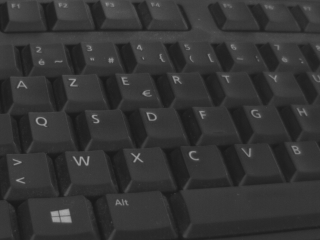
\includegraphics[width=5cm]{sobel1.png}}
\hspace{2cm}
\subfigure[Image with Sobel operator]{
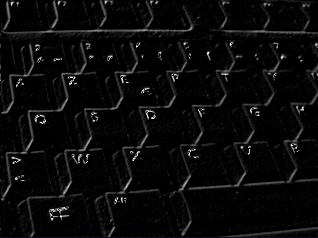
\includegraphics[width=5cm]{sobel2.png}}
\end{figure}

\vspace{0.5cm}

\section*{Equivalence}

\subsection*{Matlab}

\lstset { %
    language=Matlab,%
    %basicstyle=\color{red},
    breaklines=true,%
    morekeywords={matlab2tikz},
    keywordstyle=\color{blue},%
    morekeywords=[2]{1}, keywordstyle=[2]{\color{black}},
    identifierstyle=\color{black},%
    stringstyle=\color{mylilas},
    commentstyle=\color{mygreen},%
    showstringspaces=false,%without this there will be a symbol in the places where there is a space
    numbers=none,%
    numberstyle={\tiny \color{black}},% size of the numbers
    numbersep=9pt, % this defines how far the numbers are from the text
    emph=[1]{for,end,break, while},emphstyle=[1]\color{blue}, %some words to emphasise
    %emph=[2]{word1,word2}, emphstyle=[2]{style}, 
}
\begin{lstlisting}
%% Matlab - Sobel edge detection

I = imread('cell.tif');
figure, imshow(I), title('Original image');
SOBEL = edge(I, 'sobel');
figure, imshow(SOBEL)

\end{lstlisting}


\subsection*{OpenCV}

\lstset { %
    language=Matlab,%
    %basicstyle=\color{red},
    breaklines=true,%
    morekeywords={matlab2tikz},
    keywordstyle=\color{blue},%
    morekeywords=[2]{1}, keywordstyle=[2]{\color{black}},
    identifierstyle=\color{black},%
    stringstyle=\color{mylilas},
    commentstyle=\color{mygreen},%
    showstringspaces=false,%without this there will be a symbol in the places where there is a space
    numbers=none,%
    numberstyle={\tiny \color{black}},% size of the numbers
    numbersep=9pt, % this defines how far the numbers are from the text
    emph=[1]{for,end,break, while},emphstyle=[1]\color{blue}, %some words to emphasise
    %emph=[2]{word1,word2}, emphstyle=[2]{style}, 
}
\begin{lstlisting}
/// OpenCV - Sobel edge detection

/// Gradient X
  Sobel( src_gray, grad_x, ddepth, 1, 0, 3, scale, delta, BORDER_DEFAULT );
  convertScaleAbs( grad_x, abs_grad_x );

/// Gradient Y
  Sobel( src_gray, grad_y, ddepth, 0, 1, 3, scale, delta, BORDER_DEFAULT );
  convertScaleAbs( grad_y, abs_grad_y );

/// Total Gradient (approximate)
  addWeighted( abs_grad_x, 0.5, abs_grad_y, 0.5, 0, grad );

\end{lstlisting}

\newpage

\section*{Mathematical formalism}

The operator uses 2 $3x3$ kernels which are convolved with the original image to compute approximations of the horizontal and vertical derivatives. \\

If we define $I$ as the source image, $\bigtriangledown_x$ and $\bigtriangledown_y$ as the horizontal and vertical derivative approximation respectively. $\bigtriangledown_x$ and $\bigtriangledown_y$ are written as follows :\\

\begin{equation}\label{eq1}
\bigtriangledown_x = \begin{pmatrix}
-1 & 0 & 1 \\ 
-2 & 0 & 2 \\ 
-1 & 0 & 1
\end{pmatrix}*I
\end{equation}

\vspace{0.5cm}

\begin{equation}\label{eq2}
\bigtriangledown_y = \begin{pmatrix}
-1 & -2 & -1 \\ 
0 & 0 & 0 \\ 
1 & 2 & 1
\end{pmatrix}*I
\end{equation}

\vspace{0.5cm}

We can develop (\ref{eq1}) and (\ref{eq2}) as follows :\\

\begin{equation}\label{eq3}
\begin{matrix}
\bigtriangledown_x = \begin{pmatrix}
-1 & 0 & 1 \\ 
-2 & 0 & 2 \\ 
-1 & 0 & 1
\end{pmatrix}*I  = \begin{pmatrix}
-1 & 0 & 1 \\ 
-2 & 0 & 2 \\ 
-1 & 0 & 1
\end{pmatrix}* \begin{pmatrix}
i_{00} & i_{01} & i_{02} \\ 
i_{10} & i_{11} & i_{12}\\ 
i_{20} & i_{21} & i_{22}
\end{pmatrix}  \\ 
& & \\
 =  -i_{00}-2i_{10}-i_{20}+i_{02}+2i_{12}+i_{22} \\ 
\end{matrix}
\end{equation}

\vspace{1cm}

\begin{equation}\label{eq4}
\begin{matrix}
\bigtriangledown_y = \begin{pmatrix}
-1 & -2 & -1 \\ 
0 & 0 & 0 \\ 
1 & 2 & 1
\end{pmatrix}*I  = \begin{pmatrix}
-1 & -2 & -1 \\ 
0 & 0 & 0 \\ 
1 & 2 & 1
\end{pmatrix}* \begin{pmatrix}
i_{00} & i_{01} & i_{02} \\ 
i_{10} & i_{11} & i_{12}\\ 
i_{20} & i_{21} & i_{22}
\end{pmatrix}  \\ 
& & \\
 =  -i_{00}-2i_{01}-i_{02}+i_{20}+2i_{21}+i_{22} \\ 
\end{matrix}
\end{equation}
 
\vspace{0.5cm}

In each point, we give an approximation of the gradient norm by the equation (\ref{eq5})

\begin{equation}\label{eq5}
\bigtriangledown = \sqrt{\bigtriangledown_x^2 + \bigtriangledown_y^2 } \simeq \bigtriangledown_x + \bigtriangledown_y
\end{equation}

\vspace{0.5cm}

Thus, we obtain :

\begin{equation}\label{eq6}
\bigtriangledown \simeq 2(i_{12}+i_{22}+i_{21}-i_{00}-i_{10}-i_{01})
\end{equation}
 
\vspace{0.25cm}
 
And finally in matrix form : 

\begin{equation}\label{eq7}
\kappa_S  \simeq \begin{pmatrix}
-2 & -2 & 0\\ 
-2 & 0 & 2\\ 
 0 & 2 & 2
\end{pmatrix}
\end{equation}

\end{document}